\documentclass[12pt,letterpaper]{report}
\usepackage[spanish]{babel}
\usepackage[utf8]{inputenc}
\usepackage{graphicx}


\begin{document}

\section{Retinopatía}\label{cap.retinopatia}
\subsection{Síntomas y causas.}
Las causa principal de este padecimiento es el cambio en la circulación de la sangre con la que cuentan las personas que padecen diabetes principalmente el aumento de la glucosa, dañando así los vasos sanguíneos que se encuentran en la retina causando hemorragias, perdida de liquido y acumulación de grasas en la zona del ojo.\\

Los factores causantes de esto que se catalogan como modificables, son:
\begin{itemize}
\item Cantidad de glucosa en la sangre.
\item Nivel de presión arterial.
\item Niveles de lípidos en sangre.
\end{itemize}
Son factores que con un control cotidiano y un estilo de vida saludable del paciente pueden no ser causantes de crear el ambiente para el desarrollo de la retinopatía.

En el caso de los factores no modificables como es:

\begin{itemize}
\item Tiempo de padecer diabetes.
\item Edad del paciente.
\item Predisposición genética.
\item Embarazo (En caso de pacientes femeninos).
\end{itemize}

%Citar pagina de internet https://www.clinicbarcelona.org/asistencia/enfermedades/retinopatia-diabetica/causas-y-factores-de-riesgo#:~:text=La%20retinopat%C3%ADa%20diab%C3%A9tica%20est%C3%A1%20causada,l%C3%ADquido%20y%20c%C3%BAmulo%20de%20grasas.%


En las etapas tempranas de la enfermedad, los pacientes no muestran sintomas de importancia, lo que va cambiando conforme avanza el grado de daño producido.\\

Los pacientes pueden presentar: 
\begin{itemize}
\item Manchas o hebras oscuras que flotan en la vista (moscas volantes)
\item Visión borrosa
\item Visión variable
\item Visión de colores alterada
\item Zonas de la visión oscura o vacía
\item Pérdida de la visión
\end{itemize}

%Citar doi 10.26820/recimundo/5.(3).sep.2021.397-404



\subsection{Tipos de retinopatía.}
\begin{itemize}

\item \textbf{Sin retinopatía aparente.}\\
\linebreak 
No se observan lesiones características al examen oftalmoscópico.
\medskip

\item \textbf{Retinopatía no proliferante leve.}\\
\linebreak
Sólo se encuentran microaneurisma retinianos, como primera alteración apreciable oftalmoscópicamente de RD. Los microaneurismas son dilataciones de la pared de los capilares y aparecen como puntos rojos pequeños de bordes muy nítidos.


\medskip\
\item \textbf{Retinopatía diabética no proliferante moderada.}
\\
\linebreak
Aparecen hemorragias retinianas en número inferior a 20 en los cuatro cuadrantes. Pueden existir exudados duros o lipídicos y blandos o algodonosos (Fig. 2.1) y además dilataciones venosas arrosariadas en un solo cuadrante. Las dilataciones venosas consisten en zonas bien localizadas de dilatación con zonas de estrechez venosa, como cuentas de un rosario. El trayecto venoso se vuelve tortuoso y en ocasiones parece bifurcado.


\begin{figure}[!htb]
    \centering
    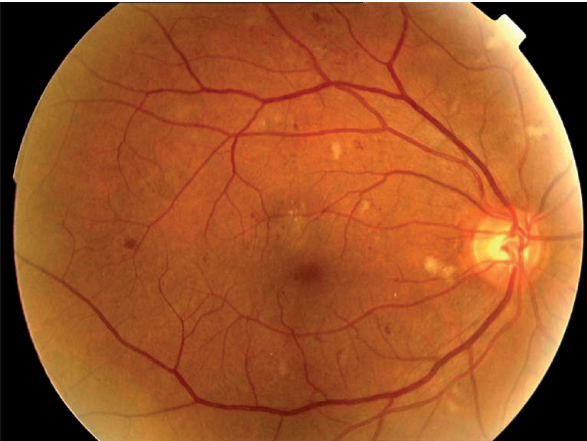
\includegraphics[width=.75\textwidth]{Img_C2_2.1/FIG_1.png} 
    \caption{Retinopatía diabética no proliferante moderada.}
    \label{fig:fig1}
\end{figure}

\medskip
\item \textbf{Retinopatía diabética no proliferante severa.}\\\
\linebreak
Pueden presentarse cualquiera de las siguientes alteraciones: hemorragias intrarretinianas severas en número superior a 20 en cada uno de los cuatro cuadrantes (Fig. 2.2), o dilataciones venosas arrosariadas en 2 ó más cuadrantes, o anomalías microvasculares intrarretinianas (IRMA) bien definidas en un cuadrante. El riesgo de progresión a RD proliferante es del 50.2\% en un año. Y de RD proliferante de alto riesgo 14.6\%, si se dan la regla completa este riesgo será del 45\% en un año.
\linebreak

\begin{figure}[!htb]
    \centering
    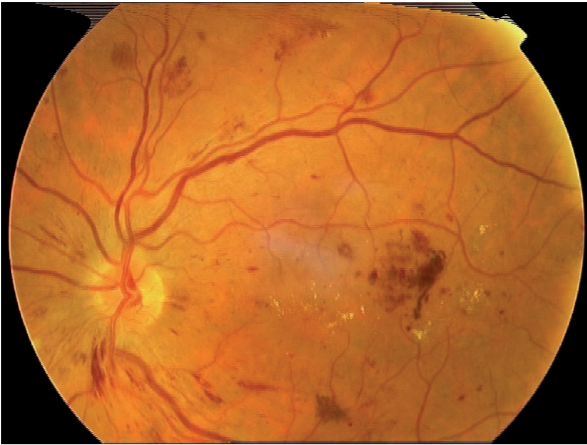
\includegraphics[width=.75\textwidth]{Img_C2_2.1/FIG_2.png}  
    \caption{Retinopatía diabética no proliferante severa.}
    \label{fig:fig2}
\end{figure}

\pagebreak
\item \textbf{Retinopatía diabética proliferante.}\\\
\linebreak
Incluye toda neovascularización retiniana o papilar (Fig. 2.3) bien definida y/o hemorragia vítrea o prerretiniana extensa. (Incluye los niveles 61 y 65 como formas leves o moderadas de neovascularización, y el 71 a 85 como formas de alto riesgo y avanzadas con proliferación fibrovascular (Fig. 2.4) y desprendimiento de retina traccional). En este nivel de severidad la fotocoagulación láser (Fig. 2.5) será necesaria para controlar la evolución, en el caso de neovasos en el disco extensos o hemorragia vítrea y será necesaria de manera inmediata.
\medskip
\linebreak

\begin{figure}[p]
    \centering
    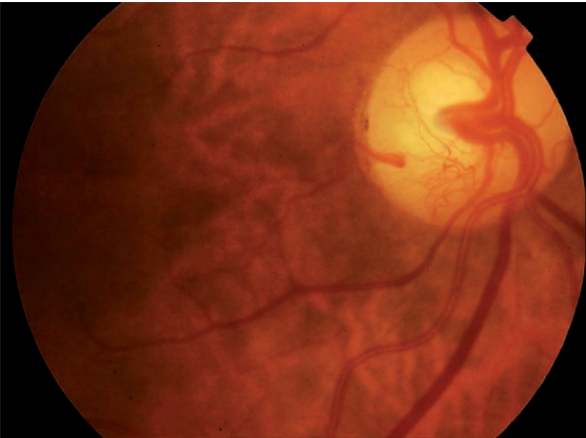
\includegraphics[width=.75\textwidth]{Img_C2_2.1/FIG_3.png}  
    \caption{Retinopatía proliferante donde se observan claramente los neovasos papilares.}
    \label{fig:fig3}
\end{figure}

\begin{figure}
    \centering
    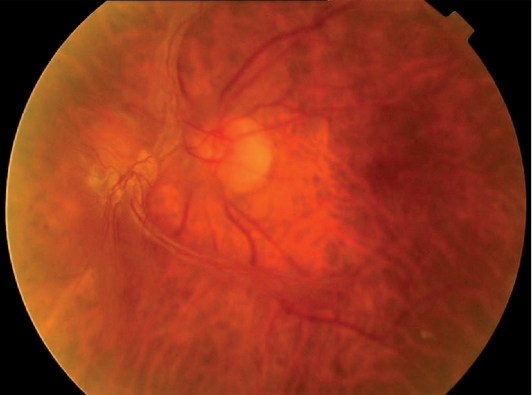
\includegraphics[width=.75\textwidth]{Img_C2_2.1/FIG_4.png} 
    \caption{Retinopatía proliferante. Existe proliferación fibrovascular con tracción retiniana y sobre la
papila.}
    \label{fig:fig4}
\end{figure}
\medskip
\begin{figure}
    \centering
    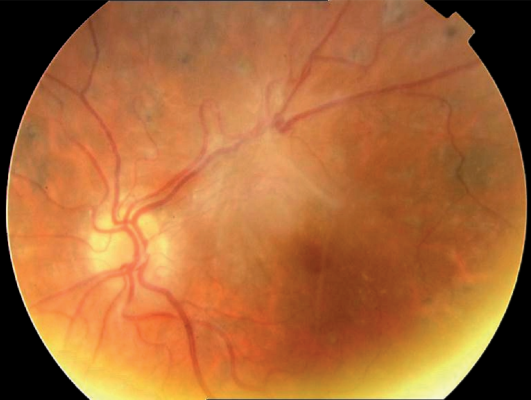
\includegraphics[width=.75\textwidth]{Img_C2_2.1/FIG_5.png} 
    \caption{Retinopatía proliferante. Se pueden observar las cicatrices pigmentadas de la panfotocoagulación}
    \label{fig:fig5}
\end{figure}
\end{itemize}
%Todos parrafos y fotos del 2.1.2 debe citar ALISEDA, D.; BERÁSTEGUI, L. Retinopatía diabética. En Anales del sistema sanitario de Navarra. Gobierno de Navarra. Departamento de Salud, 2008. p. 25-28.
\pagebreak
\subsection{Tratamiento.}

En la actualidad contamos con una terapia quirúrgica la cual hace uso del láser en conjunto de una terapia farmacológica utilizando agentes anti-VEFG de manera repetitiva mensual, haciendo que reduzca la progresión de la retinopatía en un 25\%-30\% en pacientes tratados durante 2 años con ambas terapias, en comparación de pacientes los cuales únicamente usaron la terapia láser por separado.

El significativo progreso en el manejo de la retinopatía, se ha logrado gracias al avance de las imágenes oculares, la tomografía de coherencia óptica la cual permite la detección anatómica temprana de los cambios en la mácula, del engrosamiento retiniano y de la formación de quistes en el edema macular diabético.
%cita http://repository.urosario.edu.co/handle/10336/18648 paginas 43-45

Dentro de las terapias en estudio, se pueden nombrar las siguientes: el uso de la somatostatina este es un neuro protector anti-angiogénico, este se encuentra en estudios en fase II y III; el péptido semejante al Glucagón es un neuro-protector, su aplicación intravítrea, previene la neurodegeneración retiniana en ratas con diabetes.\\
\linebreak
La doxiciclina es un antiinflamatorio y neuro-protector que mejora la función de la retina interna comparado con placebo, se han obtenido resultados estadísticamente significativos, pero se reporta en muestra muy pequeña para generalizar los resultados.
%cita http://repository.urosario.edu.co/handle/10336/18648 paginas 43-45
\pagebreak
\end{document}
